\documentclass[11pt,fleqn]{article}

\setlength {\topmargin} {-.15in}
\setlength {\textheight} {8.6in}

\usepackage{amsmath}
\usepackage{amssymb}
\usepackage{color}
\usepackage{tikz}
\usetikzlibrary{automata,positioning,arrows}
\usepackage{diagbox}



\newcommand{\be}{\begin{enumerate}}
\newcommand{\ee}{\end{enumerate}}

\begin{document}

\textbf{Exercise 4.2.24:} Hamiltonian path in DAGs. Given a DAG, design a linear-time algorithm to
determine whether there is a directed path that visits each vertex exactly once.\\

\textbf{Solution:}\\
Recall Hamiltonian path is a path that visits every $vertex$ atmost exactly once. Eulers path reaches every $edge$ exactly once but can pass through a vertex more than once(since vertices may well be crossed more than once). So Hamiltonian is mainly for vertices while eulers is more for reachability of edges.\\

Something like 0,1,2,3,4,5,6 is a VALID path, Topological path, and a hamiltonian path.\\

Good concept: If we do topological sort and see direct edge between 2 nodes, then it is a hamiltonian path. We can't have edge going in opposite direction for topological order(TO). If only one unique path topological order, then it is a Hamiltonian path. If you have consecutive edges, then also a Hamiltonian path.

\begin{center}
	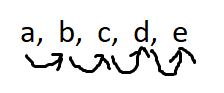
\includegraphics[scale=1]{4.2.24.png}
\end{center}

	


\end{document}
